\begin{itemize}
\item Claim1: Uniform quantization matches the performance of complex methods
	\begin{itemize}
		\item Figures on 4 tasks: DrQa, one sentiment, one word analogy and one word similarity
		\item Tables on tasks performance and time
	\end{itemize}
\item Claim 2: Subspace overlap characterize compressed embedding on downstream task performance.
	\begin{itemize}
		\item Figures on correlation between performance and Overlap, pip loss, delta1 and delta 2 (potentially use max(1/(1-delta1), delta2)) for all the tasks?
		\item Can check out to see if we can do R2 measurements reliably
	\end{itemize}
\end{itemize}

%We now evaluate the performance of our word embedding compression algorithm on a variety of NLP tasks (question answering, sentiment analysis, word analogy/similarity) and embeddings types (GloVe, fastText).
%We present two main conclusions:
%(1) Uniform quantization is consistently able to match the performance of more complex baselines (DCCL, k-means), while dramatically outperforming a more naive dimensionality reduction baseline (\S\ref{sec:exp_comparison});
%(2) When considering a fixed memory budget, low-precision high-dimensional embeddings significantly outperform high-precision low-dimensional embeddings (\S\ref{sec:dim_vs_prec}).
%%We observe that in this memory-constrained setting, the best compressed embeddings attain \todo{XX\%} to \todo{YY\%} better performance than the full-precision embeddings.
%This demonstrates the importance of considering low-precision when trying to attain the best possible performance under a memory budget.
%
%For extended details about all of our experiments, and for results which did not fit in the main text, please see Appendix~\ref{app:experiments}.
%
%\subsection{Empirical Comparison of Compression Methods}
%\label{sec:exp_comparison}
%%\begin{itemize}
%%	\item \textbf{Embeddings}: GloVe ($d\in\{50,100,200,300\}$, $n=400k$) and fastText ($d=300$, $n=10^6$) pre-trained.
%%	\item \textbf{Baselines}: k-means, DCCL, dim. reduction (GloVe)
%%	\item \textbf{Tasks}: DrQA, sentiment, intrinsics, synthetics.
%%	\item \textbf{Compression ratios}: 8x-32x.
%%	\item \textbf{Number of random seeds}: 5
%%\end{itemize}
%In this section, we show that across a variety of tasks and embedding types, uniform quantization performs comparably to the DCCL and k-means compression methods, while significantly outperforming a dimensionality reduction baseline.
%Specifically, in Figure~\ref{fig:comparison_results} we compare the performance of these compression methods on publicly available pre-trained GloVe and fastText embeddings,\footnote{We use the Wikipedia 2014 + Gigaword 5 GloVe embeddings available at \url{http://nlp.stanford.edu/data/glove.6B.zip}, and the 300-dimensional fastText embeddings trained on Wikipedia 2017, UMBC webbase corpus and statmt.org news dataset, available at \url{https://s3-us-west-1.amazonaws.com/fasttext-vectors/wiki-news-300d-1M.vec.zip}}
%on four types of NLP tasks (question answering, sentiment analysis, word analogy, word similarity).
%For the dimensionality reduction baseline, we evaluate the performance of the lower-dimensional pre-trained GloVe embeddings ($d\in\{50,100,200,300\}$, and compare their performance to the compressed 300-dimensional embeddings.
%We use five random seeds per compression configuration, and plot the average performance per task, using error bars to denote the standard deviation.
%\todo{Reorganize this a bit, to put explanation of tasks before the results.}
%
%We now provide some details on how we performed each of these evaluations; for more information, please see Appendix~\ref{app:experiment_details}.
%For the question answering task, we train the DrQA model \citep{drqa17} on the Stanford Question Answering Dataset (SQuAD 1.1) \citep{squad16}.
%For the sentiment analysis task, we train the convolutional neural network (CNN) architecture proposed by \citet{kim14} on a number of sentiment analysis datasets; we plot results for the TREC dataset in Figure~\ref{fig:comparison_results}, but include results across all datasets in Appendix~\ref{app:experiment_results}.
%For the word analogy and similarity results, we evaluate on the same tasks as \citet{levy15}, and use their code repository for the evaluation.
%In Figure~\ref{fig:comparison_results}(c,d) we plot the average performance across the various word analogy and similarity tasks, respectively.
%
%%\begin{figure}
%%\begin{center}
%%\centerline{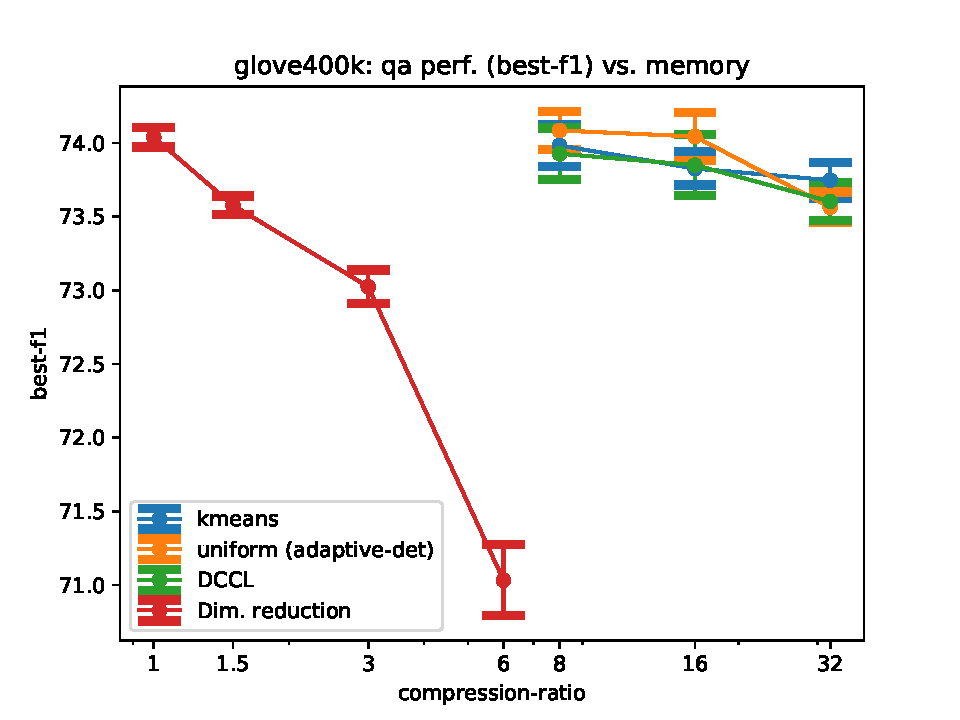
\includegraphics[width=\columnwidth]{figures/glove400k_qa_best-f1_vs_compression.pdf}}
%%\caption{Question answering performance (DrQA) for a number of compression methods at various compression ratios, on pre-trained GloVe embedding.  Uniform quantization performs similarly to k-means and DCCL, while significantly outperforming the dimensionality reduction baseline. \todo{TODO: Include fastText results (though there won't be a dim. reduction baseline, since they don't release pre-trained embeddings at smaller dimensions.)}}
%%\label{fig:glove400k_drqa}
%%\end{center}
%%\end{figure}
%
%
%\begin{figure*}
%	\centering
%	%	\begin{tabular}{c c c c}
%	\begin{tabular}{@{\hskip -0.0in}c@{\hskip -0.0in}c@{\hskip -0.0in}c@{\hskip -0.0in}c@{\hskip -0.0in}}
%		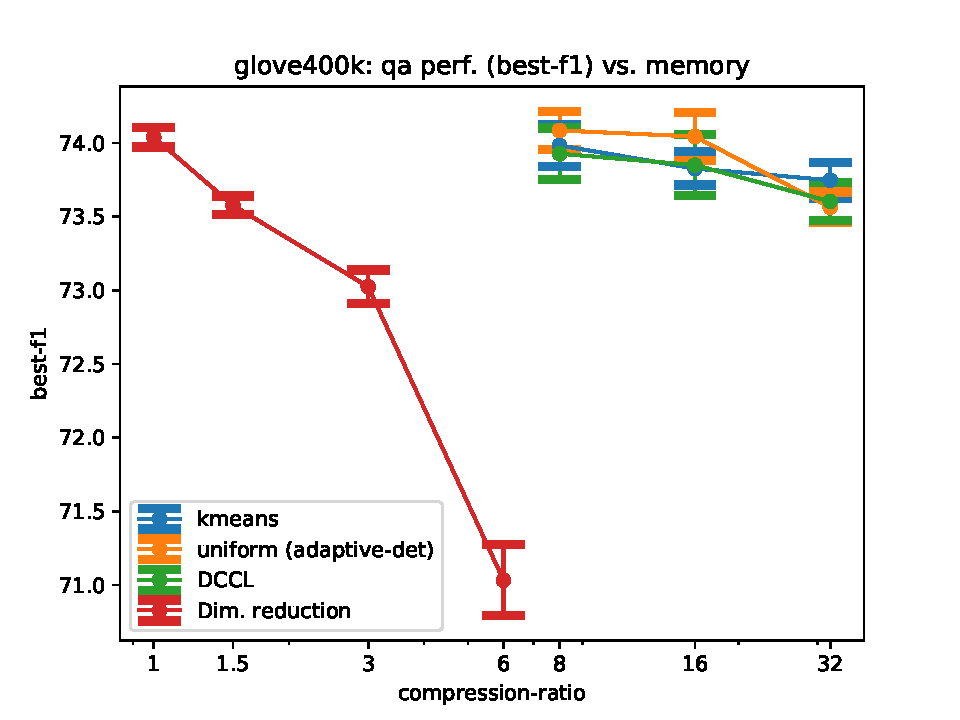
\includegraphics[width=.245\linewidth]{figures/glove400k_qa_best-f1_vs_compression.pdf} &
%		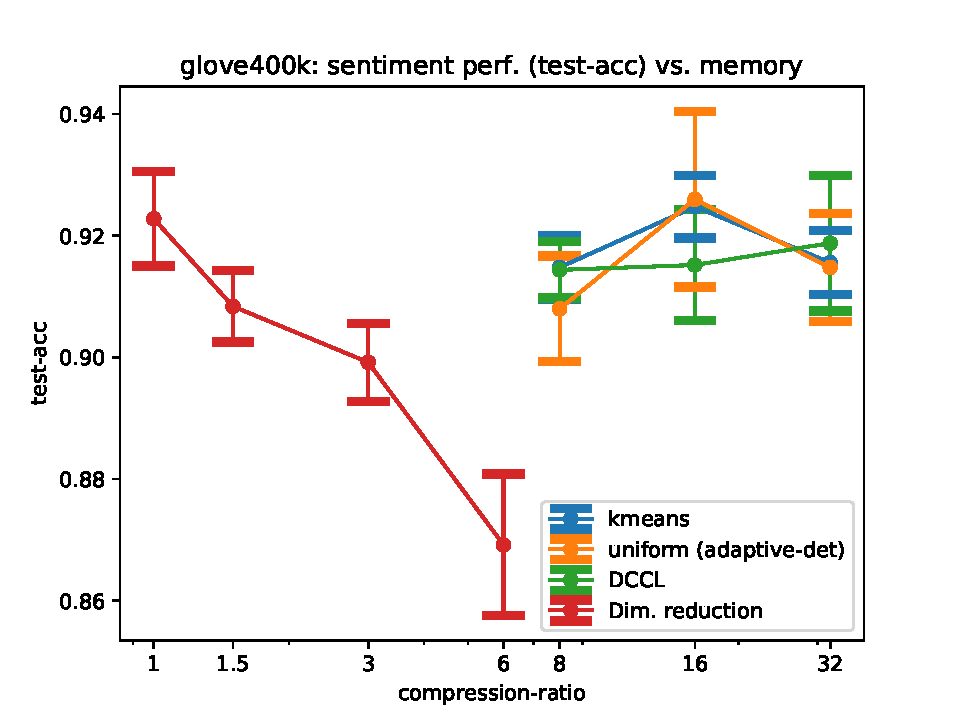
\includegraphics[width=.245\linewidth]{figures/glove400k_sentiment_trec_test-acc_vs_compression.pdf} &
%		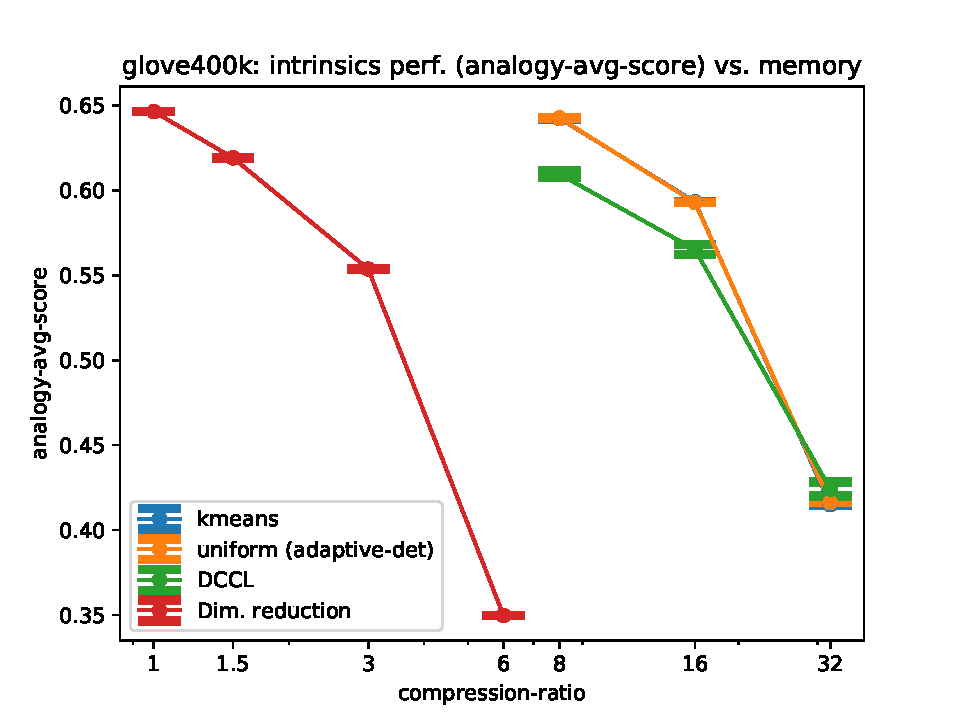
\includegraphics[width=.245\linewidth]{figures/glove400k_intrinsics_analogy-avg-score_vs_compression.pdf} &
%		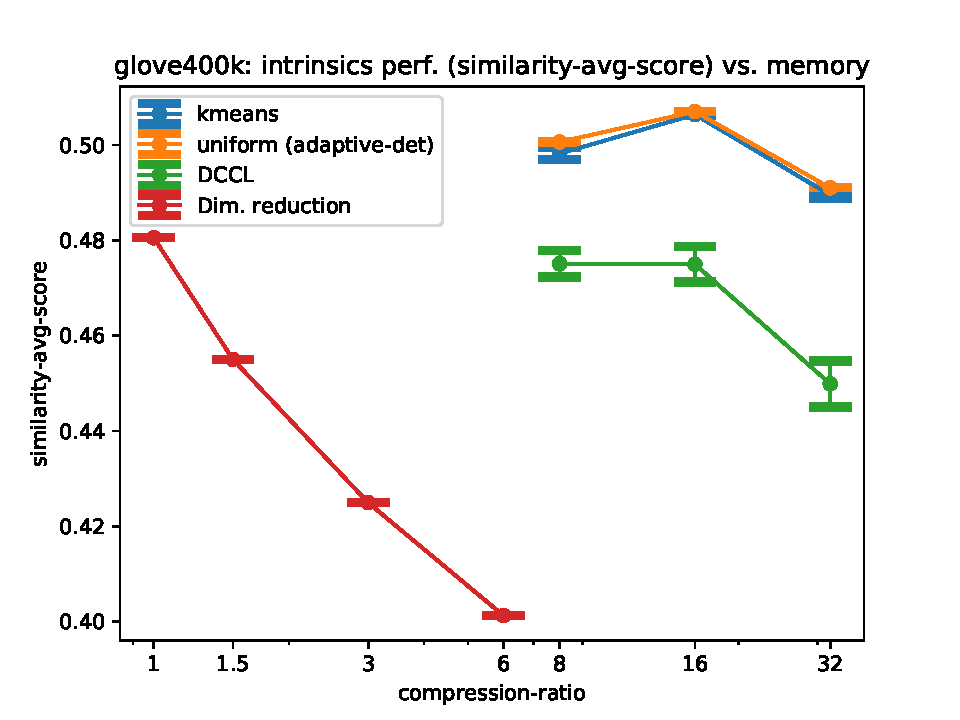
\includegraphics[width=.245\linewidth]{figures/glove400k_intrinsics_similarity-avg-score_vs_compression.pdf} \\
%		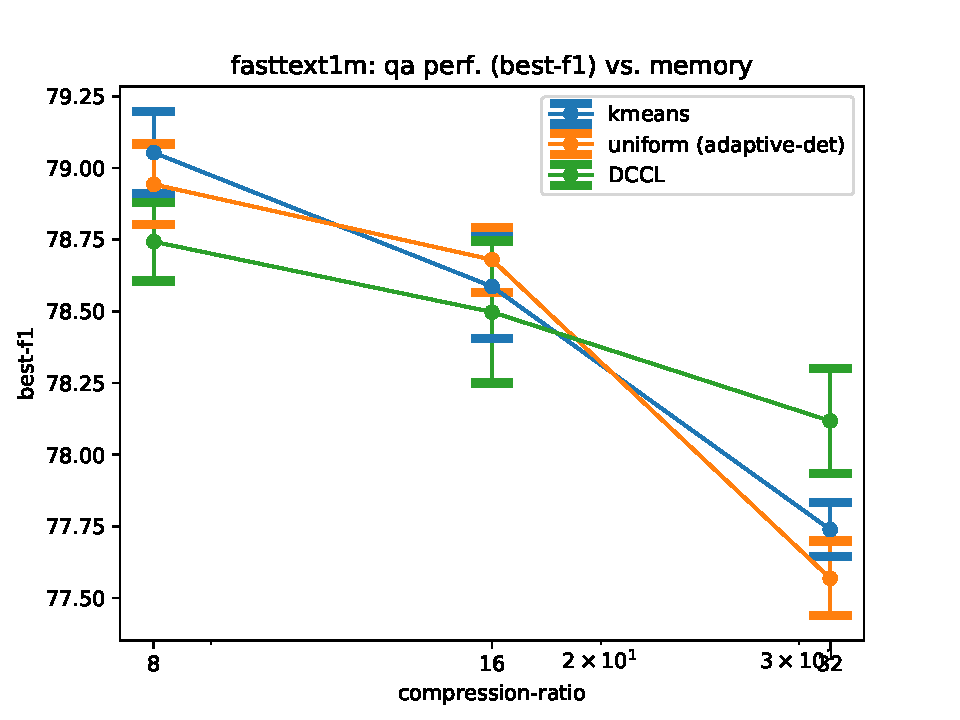
\includegraphics[width=.245\linewidth]{figures/fasttext1m_qa_best-f1_vs_compression.pdf} &
%		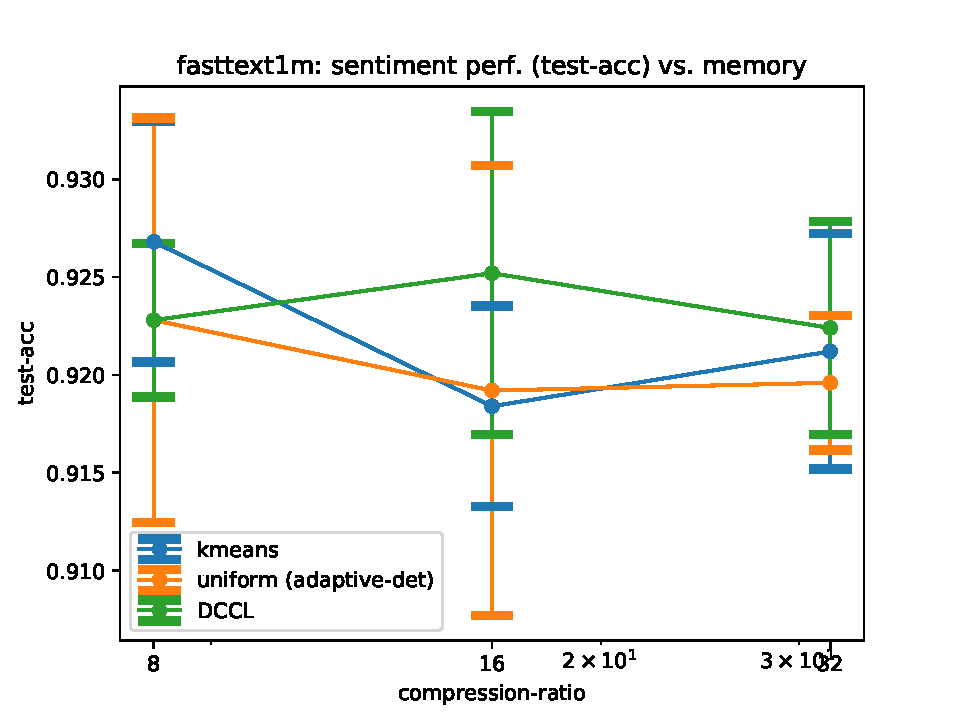
\includegraphics[width=.245\linewidth]{figures/fasttext1m_sentiment_trec_test-acc_vs_compression.pdf} &
%		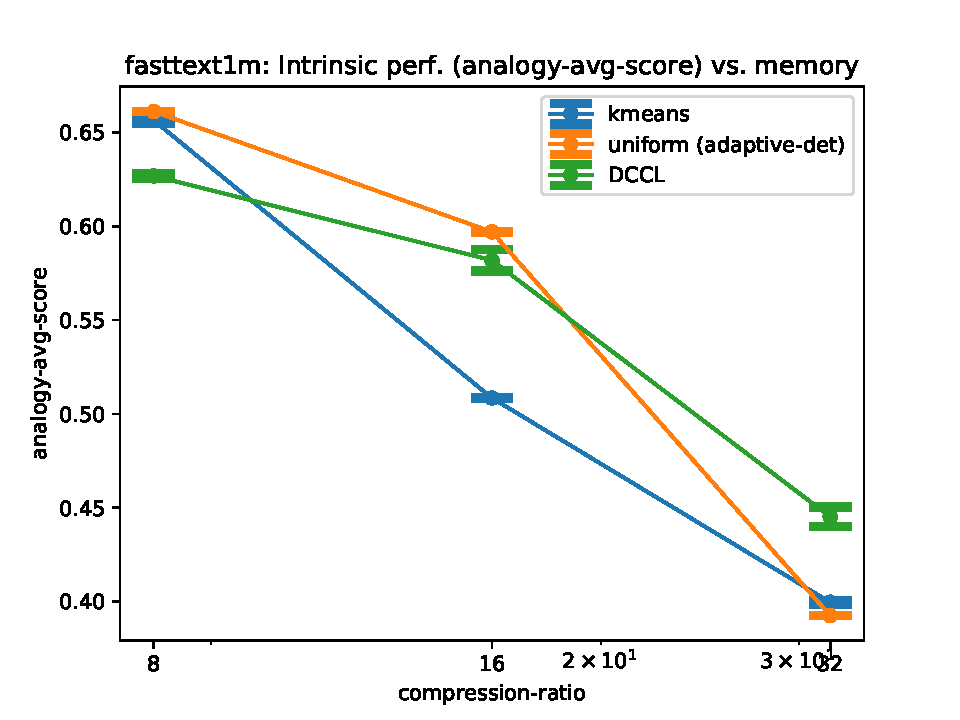
\includegraphics[width=.245\linewidth]{figures/fasttext1m_intrinsics_analogy-avg-score_vs_compression.pdf} &
%		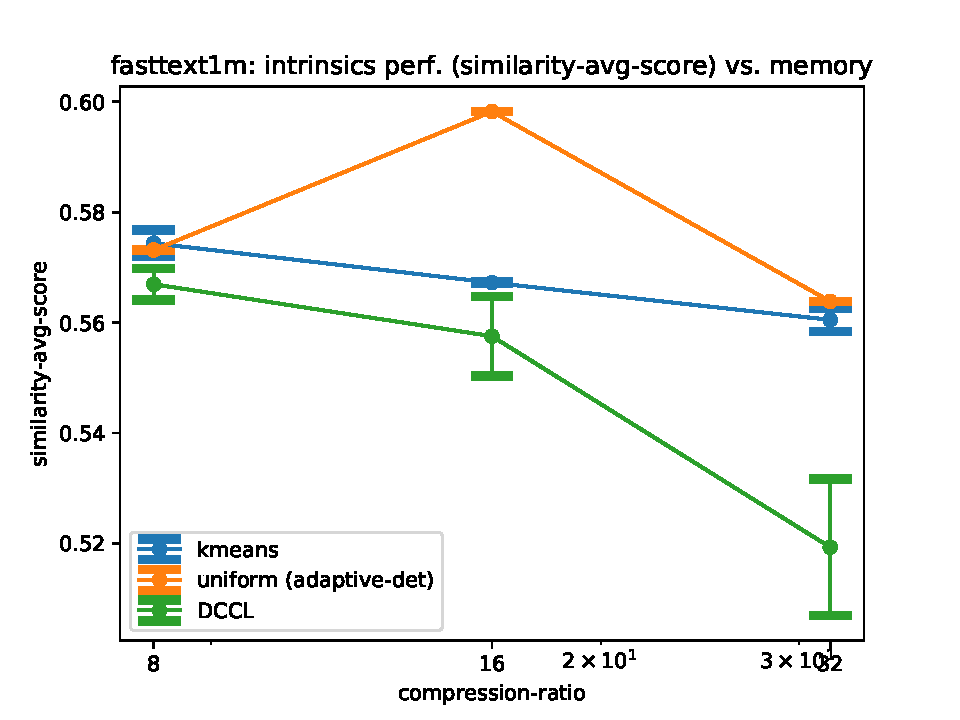
\includegraphics[width=.245\linewidth]{figures/fasttext1m_intrinsics_similarity-avg-score_vs_compression.pdf} \\
%		\;\;\;\;\;(a) & \;\;\;\;\;\;(b) & \;\;\;\;\;\;(c) & \;\;\;\;\;\;(d)
%	\end{tabular}
%\caption{Performance of compressed GloVe (top) and fastText (bottom) embeddings on question answering (a), sentiment analysis (TREC dataset) (b), word analogy (c), and word similarity (d) tasks.
%Uniform quantization performs similarly to k-means and DCCL on question answering and sentiment analysis;
%on the word analogy and similarity tasks, uniform quantization once again performs similarly to k-means, but outperforms the DCCL method.
%For the GloVe experiments, we are also able to compare with pre-trained embeddings of smaller dimensions ($d\in\{50,100,200,300\}$), and observe that compressing the 300-dimensional embeddings is significantly better than using lower-dimensional full-precision embeddings (``Dim. reduction'').
%}
%\label{fig:comparison_results}
%\end{figure*}
%
%\begin{figure*}
%	\centering
%	\begin{tabular}{@{\hskip -0.0in}c@{\hskip -0.0in}c@{\hskip -0.0in}c@{\hskip -0.0in}c@{\hskip -0.0in}}
%		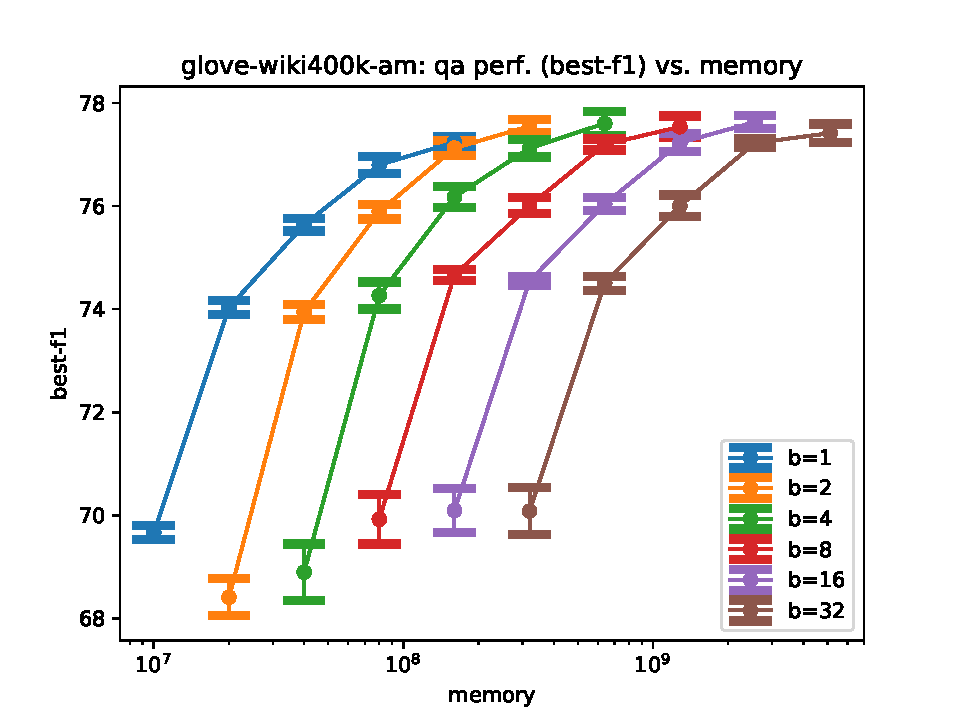
\includegraphics[width=.245\linewidth]{figures/glove-wiki400k-am_qa_best-f1_vs_compression.pdf} &
%		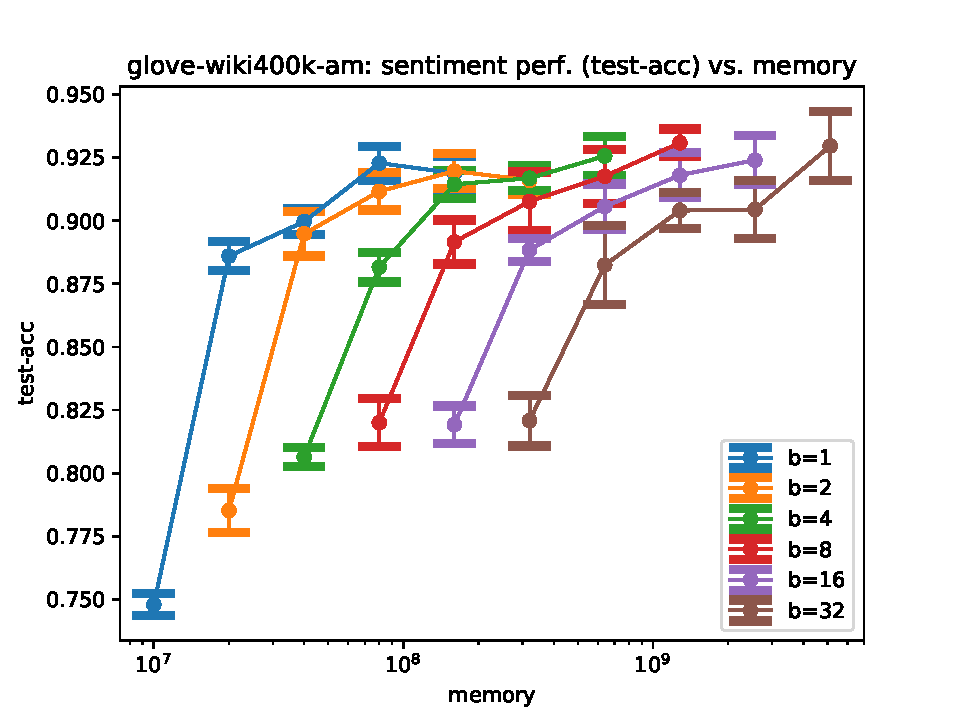
\includegraphics[width=.245\linewidth]{figures/glove-wiki400k-am_sentiment_trec_test-acc_vs_compression.pdf} &
%		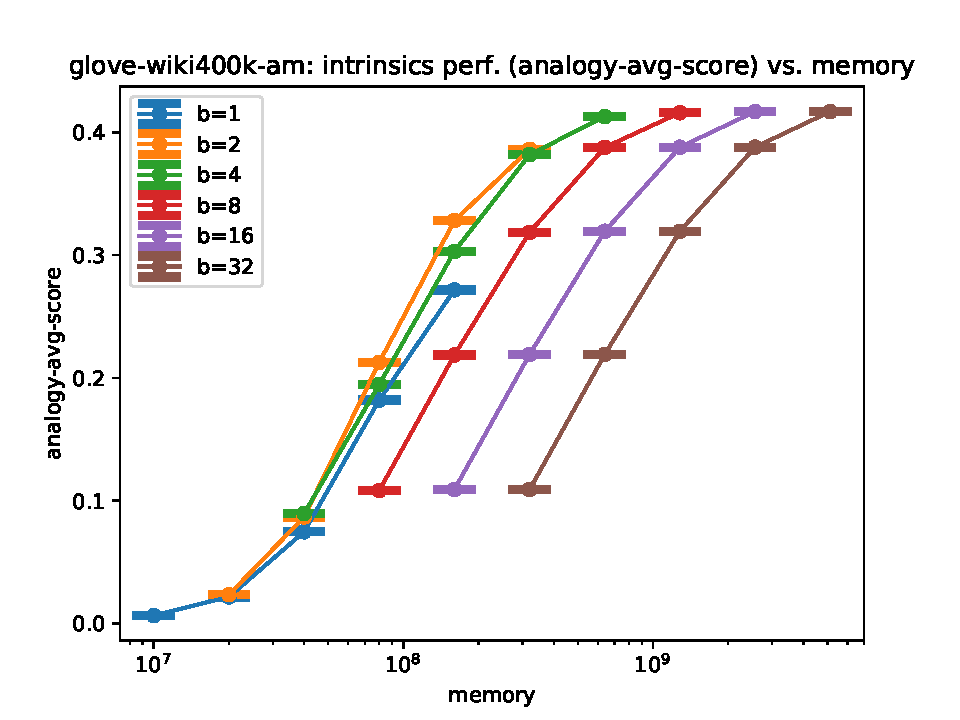
\includegraphics[width=.245\linewidth]{figures/glove-wiki400k-am_intrinsics_analogy-avg-score_vs_compression.pdf} &
%		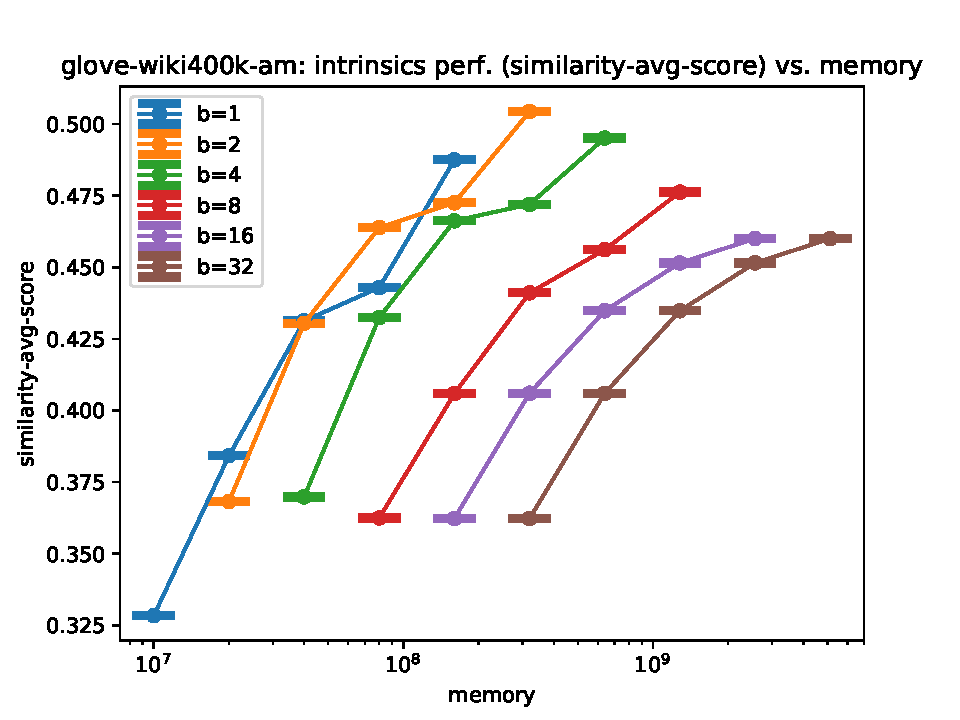
\includegraphics[width=.245\linewidth]{figures/glove-wiki400k-am_intrinsics_similarity-avg-score_vs_compression.pdf} \\
%		\;\;\;\;\;(a) & \;\;\;\;\;\;(b) & \;\;\;\;\;\;(c) & \;\;\;\;\;\;(d)
%	\end{tabular}			
%%		\begin{tabular}{@{\hskip -0.0in}c@{\hskip -0.0in}c@{\hskip -0.0in}}
%%			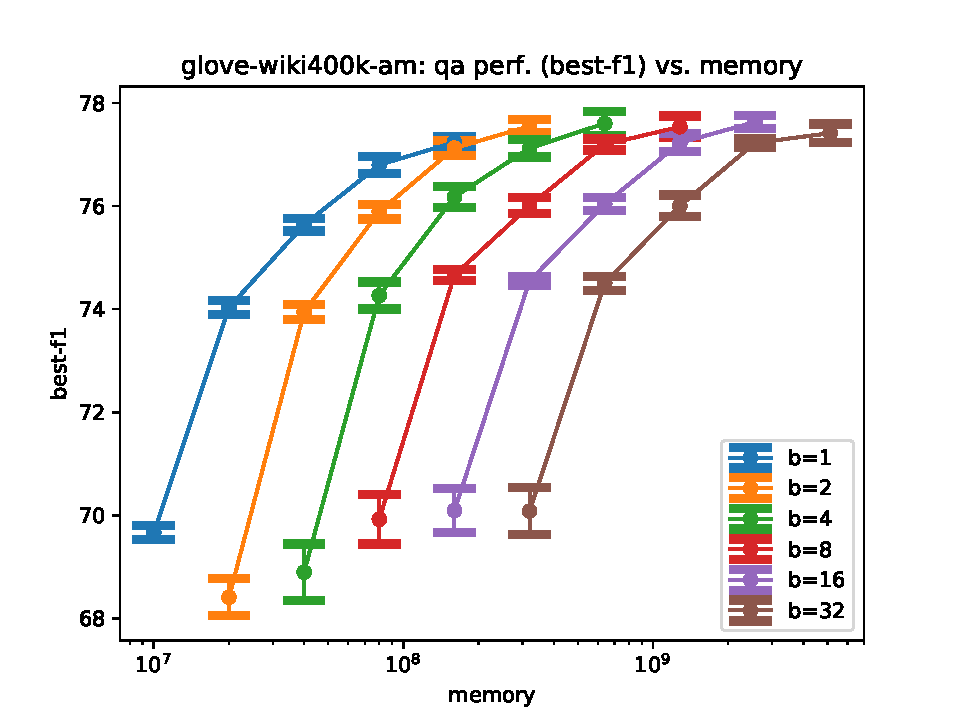
\includegraphics[width=0.4\linewidth]{figures/glove-wiki400k-am_qa_best-f1_vs_compression.pdf} &
%%			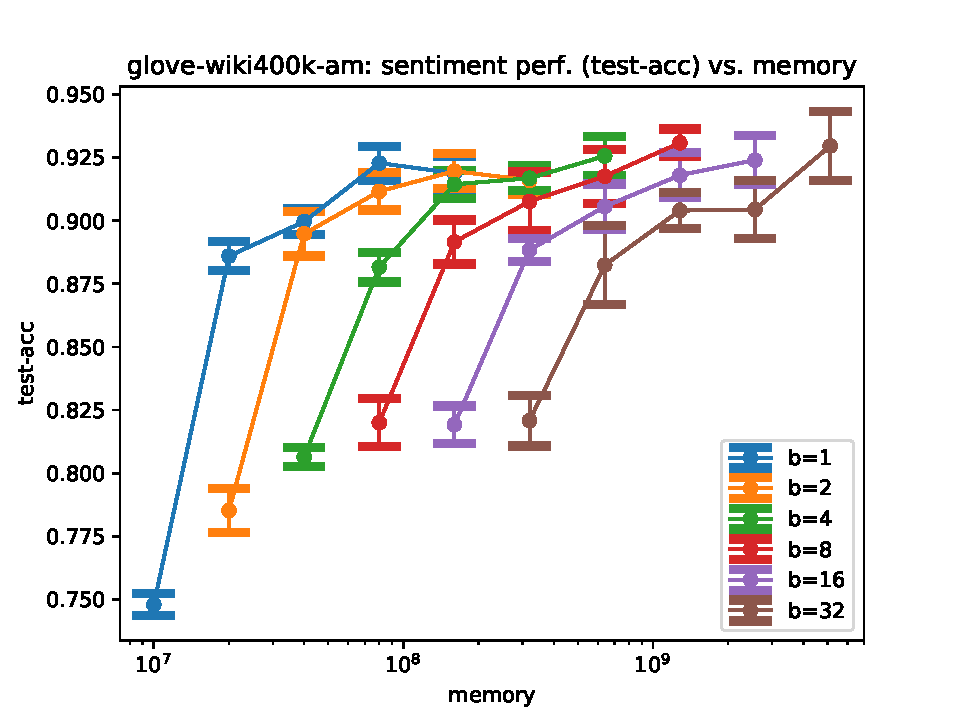
\includegraphics[width=0.4\linewidth]{figures/glove-wiki400k-am_sentiment_trec_test-acc_vs_compression.pdf} \\
%%			\;\;\;\;\;(a) & \;\;\;\;\;\;(b) 
%%		\end{tabular}
%\caption{
%Performance of GloVe embeddings of various dimensions ($d\in\{25,50,100,200,400\}$) compressed with uniform quantization for precisions $b \in \{1,2,4,8,16,32\}$, on question answering (a), sentiment analysis (TREC dataset) (b), word analogy (c), and word similarity (d) tasks.
%Here we see that when considering a memory budget, it is best to use low-precision features with high-dimensional embeddings.}
%\label{fig:dimVsPrec}
%\end{figure*}
%
%%\begin{figure*}
%%	\centering
%%	\begin{small}
%%		%		\begin{tabular}{c c c c}
%%		\begin{tabular}{@{\hskip -0.0in}c@{\hskip -0.0in}c@{\hskip -0.0in}}
%%			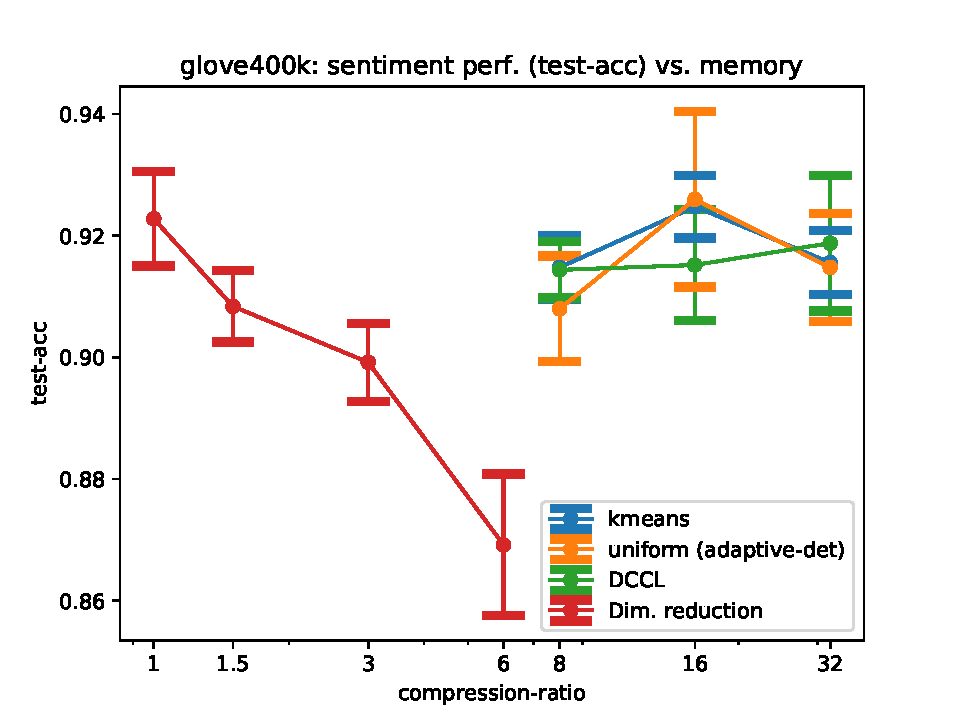
\includegraphics[width=0.45\linewidth]{figures/glove400k_sentiment_trec_test-acc_vs_compression.pdf} &
%%			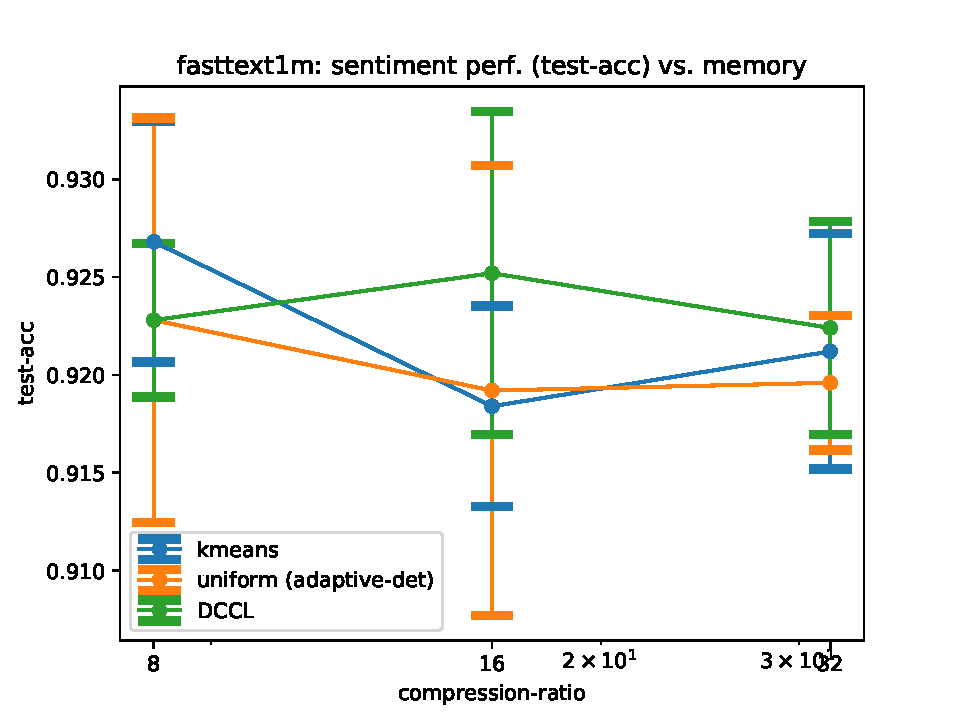
\includegraphics[width=0.45\linewidth]{figures/fasttext1m_sentiment_trec_test-acc_vs_compression.pdf} \\
%%			\;\;\;\;\;(a) & \;\;\;\;\;\;(b) 
%%		\end{tabular}
%%	\end{small}
%%	\caption{Sentiment analysis results (TREC dataset).}
%%	\label{fig:sentiment}
%%\end{figure*}
%
%\subsection{Dimension vs. Precision Trade-off}
%\label{sec:dim_vs_prec}
%%\begin{itemize}
%%	\item \textbf{Embeddings}: We train GloVe embeddings on a Wiki 2017 dump, for $n=400k$ and $d \in \{25,50,100,200,400,800\}$.
%%	\item \textbf{Bitrates}: We compress embeddings for $b \in \{1,2,4,8,16,32\}$.
%%	\item \textbf{Tasks}: DrQA, sentiment, intrinsics, synthetics.
%%	\item \textbf{Number of random seeds}: 5
%%\end{itemize}
%%
%%In Figure~\ref{fig:drqa_sent_dimVsPrec}, we show that when considering a fixed memory budget, it is best to use low-precision and high-dimensions, on both question answering and sentiment analysis tasks.
%In this section, we show that when considering a fixed memory budget for uniformly quantized embeddings, low-precision high-dimensional embeddings perform significantly better than high-precision low-dimensional embeddings.
%Specifically, we train GloVe embeddings of various dimensions ($d\in\{25,50,100,200,400\}$) on a Wikipedia 2017 corpus.\footnote{We use a full English Wikimedia dump from December 4, 2017 (4.5 billion tokens) which was pre-processed by a fastText script (\url{https://github.com/facebookresearch/fastText/blob/master/get-wikimedia.sh}) while keeping the letter cases and digits.
%We consider the $400k$ most frequent words.}
%We then compress these embeddings via uniform quantization, for precisions $b\in\{1,2,4,8,16,32\}$.
%As in Section~\ref{sec:exp_comparison}, we consider performance on question answering, sentiment analysis, word analogy, and word similarity tasks, and present results in Figure~\ref{fig:dimVsPrec}.
%As we can see, across a wide-range of memory budgets, the low-precision high-dimensional embeddings outperform the higher-precision lower-dimensional embeddings of equal size.
%\todo{Mention that we think slow-spectrum explains why $b=1$ is best.}